% ******************************* PhD Thesis Template **************************
% Please have a look at the README.md file for info on how to use the template

\documentclass[a4paper,12pt,times,numbered,print,index]{PhDThesisPSnPDF}

% ******************************************************************************
% ******************************* Class Options ********************************
% *********************** See README for more details **************************
% ******************************************************************************

% `a4paper'(The University of Cambridge PhD thesis guidelines recommends a page
% size a4 - default option) or `a5paper': A5 Paper size is also allowed as per
% the Cambridge University Engineering Deparment guidelines for PhD thesis
%
% `11pt' or `12pt'(default): Font Size 10pt is NOT recommended by the University
% guidelines
%
% `oneside' or `twoside'(default): Printing double side (twoside) or single
% side.
%
% `print': Use `print' for print version with appropriate margins and page
% layout. Leaving the options field blank will activate Online version.
%
% `index': For index at the end of the thesis
%
% `draftclassic': For draft mode without loading any images (same as draft in book)
%
% `draft': Special draft mode with line numbers, images, and water mark with
% timestamp and custom text. Position of the text can also be modified.
%
% `abstract': To generate only the title page and abstract page with
% dissertation title and name, to submit to the Student Registry
%
% `chapter`: This option enables only the specified chapter and its references
%  Useful for review and corrections.
%
% ************************* Custom Page Margins ********************************
%
% `custommargin`: Use `custommargin' in options to activate custom page margins,
% which can be defined in the preamble.tex. Custom margin will override
% print/online margin setup.
%
% *********************** Choosing the Fonts in Class Options ******************
%
% `times' : Times font with math support. (The Cambridge University guidelines
% recommend using times)
%
% `fourier': Utopia Font with Fourier Math font (Font has to be installed)
%            It's a free font.
%
% `customfont': Use `customfont' option in the document class and load the
% package in the preamble.tex
%
% default or leave empty: `Latin Modern' font will be loaded.
%
% ********************** Choosing the Bibliography style ***********************
%
% `authoryear': For author-year citation eg., Krishna (2013)
%
% `numbered': (Default Option) For numbered and sorted citation e.g., [1,5,2]
%
% `custombib': Define your own bibliography style in the `preamble.tex' file.
%              `\RequirePackage[square, sort, numbers, authoryear]{natbib}'.
%              This can be also used to load biblatex instead of natbib
%              (See Preamble)
%
% **************************** Choosing the Page Style *************************
%
% `default (leave empty)': For Page Numbers in Header (Left Even, Right Odd) and
% Chapter Name in Header (Right Even) and Section Name (Left Odd). Blank Footer.
%
% `PageStyleI': Chapter Name next & Page Number on Even Side (Left Even).
% Section Name & Page Number in Header on Odd Side (Right Odd). Footer is empty.
%
% `PageStyleII': Chapter Name on Even Side (Left Even) in Header. Section Number
% and Section Name in Header on Odd Side (Right Odd). Page numbering in footer

% Uncomment to change page style
%\pagestyle{PageStyleII}

% ********************************** Preamble **********************************
% Preamble: Contains packages and user-defined commands and settings
% ******************************************************************************
% ****************************** Custom Margin *********************************

% Add `custommargin' in the document class options to use this section
% Set {innerside margin / outerside margin / topmargin / bottom margin}  and
% other page dimensions
\ifsetCustomMargin
  \RequirePackage[left=37mm,right=30mm,top=35mm,bottom=30mm]{geometry}
  \setFancyHdr % To apply fancy header after geometry package is loaded
\fi

% Add spaces between paragraphs
%\setlength{\parskip}{0.5em}
% Ragged bottom avoids extra whitespaces between paragraphs
\raggedbottom
% To remove the excess top spacing for enumeration, list and description
%\usepackage{enumitem}
%\setlist[enumerate,itemize,description]{topsep=0em}

% *****************************************************************************
% ******************* Fonts (like different typewriter fonts etc.)*************

% Add `customfont' in the document class option to use this section

\ifsetCustomFont
  % Set your custom font here and use `customfont' in options. Leave empty to
  % load computer modern font (default LaTeX font).
  %\RequirePackage{helvet}

  % For use with XeLaTeX
  %  \setmainfont[
  %    Path              = ./libertine/opentype/,
  %    Extension         = .otf,
  %    UprightFont = LinLibertine_R,
  %    BoldFont = LinLibertine_RZ, % Linux Libertine O Regular Semibold
  %    ItalicFont = LinLibertine_RI,
  %    BoldItalicFont = LinLibertine_RZI, % Linux Libertine O Regular Semibold Italic
  %  ]
  %  {libertine}
  %  % load font from system font
  %  \newfontfamily\libertinesystemfont{Linux Libertine O}
\fi

% *****************************************************************************
% **************************** Custom Packages ********************************

% ************************* Algorithms and Pseudocode **************************

%\usepackage{algpseudocode}


% ********************Captions and Hyperreferencing / URL **********************

% Captions: This makes captions of figures use a boldfaced small font.
%\RequirePackage[small,bf]{caption}

\RequirePackage[labelsep=space,tableposition=top]{caption}
\renewcommand{\figurename}{Fig.} %to support older versions of captions.sty


% *************************** Graphics and figures *****************************

%\usepackage{rotating}
%\usepackage{wrapfig}

% Uncomment the following two lines to force Latex to place the figure.
% Use [H] when including graphics. Note 'H' instead of 'h'
%\usepackage{float}
%\restylefloat{figure}

% Subcaption package is also available in the sty folder you can use that by
% uncommenting the following line
% This is for people stuck with older versions of texlive
%\usepackage{sty/caption/subcaption}
\usepackage{subcaption}

% ********************************** Tables ************************************
\usepackage{booktabs} % For professional looking tables
\usepackage{multirow}

%\usepackage{multicol}
%\usepackage{longtable}
%\usepackage{tabularx}


% *********************************** SI Units *********************************
\usepackage{siunitx} % use this package module for SI units


% ******************************* Line Spacing *********************************

% Choose linespacing as appropriate. Default is one-half line spacing as per the
% University guidelines

% \doublespacing
% \onehalfspacing
% \singlespacing


% ************************ Formatting / Footnote *******************************

% Don't break enumeration (etc.) across pages in an ugly manner (default 10000)
%\clubpenalty=500
%\widowpenalty=500

%\usepackage[perpage]{footmisc} %Range of footnote options


% *****************************************************************************
% *************************** Bibliography  and References ********************

%\usepackage{cleveref} %Referencing without need to explicitly state fig /table

% Add `custombib' in the document class option to use this section
\ifuseCustomBib
   \RequirePackage[square, sort, numbers, authoryear]{natbib} % CustomBib

% If you would like to use biblatex for your reference management, as opposed to the default `natbibpackage` pass the option `custombib` in the document class. Comment out the previous line to make sure you don't load the natbib package. Uncomment the following lines and specify the location of references.bib file

%\RequirePackage[backend=biber, style=numeric-comp, citestyle=numeric, sorting=nty, natbib=true]{biblatex}
%\addbibresource{References/references} %Location of references.bib only for biblatex, Do not omit the .bib extension from the filename.

\fi

% changes the default name `Bibliography` -> `References'
\renewcommand{\bibname}{References}


% ******************************************************************************
% ************************* User Defined Commands ******************************
% ******************************************************************************

% *********** To change the name of Table of Contents / LOF and LOT ************

%\renewcommand{\contentsname}{My Table of Contents}
%\renewcommand{\listfigurename}{My List of Figures}
%\renewcommand{\listtablename}{My List of Tables}


% ********************** TOC depth and numbering depth *************************

\setcounter{secnumdepth}{2}
\setcounter{tocdepth}{2}


% ******************************* Nomenclature *********************************

% To change the name of the Nomenclature section, uncomment the following line

%\renewcommand{\nomname}{Symbols}


% ********************************* Appendix ***********************************

% The default value of both \appendixtocname and \appendixpagename is `Appendices'. These names can all be changed via:

%\renewcommand{\appendixtocname}{List of appendices}
%\renewcommand{\appendixname}{Appndx}

% *********************** Configure Draft Mode **********************************

% Uncomment to disable figures in `draft'
%\setkeys{Gin}{draft=true}  % set draft to false to enable figures in `draft'

% These options are active only during the draft mode
% Default text is "Draft"
%\SetDraftText{DRAFT}

% Default Watermark location is top. Location (top/bottom)
%\SetDraftWMPosition{bottom}

% Draft Version - default is v1.0
%\SetDraftVersion{v1.1}

% Draft Text grayscale value (should be between 0-black and 1-white)
% Default value is 0.75
%\SetDraftGrayScale{0.8}


% ******************************** Todo Notes **********************************
%% Uncomment the following lines to have todonotes.

%\ifsetDraft
%	\usepackage[colorinlistoftodos]{todonotes}
%	\newcommand{\mynote}[1]{\todo[author=kks32,size=\small,inline,color=green!40]{#1}}
%\else
%	\newcommand{\mynote}[1]{}
%	\newcommand{\listoftodos}{}
%\fi

% Example todo: \mynote{Hey! I have a note}

% ******************************** Highlighting Changes **********************************
%% Uncomment the following lines to be able to highlight text/modifications.
%\ifsetDraft
%  \usepackage{color, soul}
%  \newcommand{\hlc}[2][yellow]{{\sethlcolor{#1} \hl{#2}}}
%  \newcommand{\hlfix}[2]{\texthl{#1}\todo{#2}}
%\else
%  \newcommand{\hlc}[2]{}
%  \newcommand{\hlfix}[2]{}
%\fi

% Example highlight 1: \hlc{Text to be highlighted}
% Example highlight 2: \hlc[green]{Text to be highlighted in green colour}
% Example highlight 3: \hlfix{Original Text}{Fixed Text}

% *****************************************************************************
% ******************* Better enumeration my MB*************
\usepackage{enumitem}

% ******************* Comments and TODOs *************
\usepackage{todonotes} % for comments
\newcommand{\dtd}[1]{\todo[inline,color=blue!20!white]{\textbf{Daniele:} #1}}

% ******************* SI Units *************
\DeclareSIUnit{\elevationunit}{m\,a.m.s.l.}
\DeclareSIUnit{\celsius}{^\circ~C}

% ************************ Thesis Information & Meta-data **********************
% Thesis title and author information, refernce file for biblatex
% ************************ Thesis Information & Meta-data **********************
%% The title of the thesis
\title{Hydropower energy supply chain toward a sustainable water-energy nexus management}
%\texorpdfstring is used for PDF metadata. Usage:
%\texorpdfstring{LaTeX_Version}{PDF Version (non-latex)} eg.,
%\texorpdfstring{$sigma$}{sigma}

%% Subtitle (Optional)
\subtitle{Using the CUED template}

%% The full name of the author
\author{Daniele Dalla Torre}

%% Department (eg. Department of Engineering, Maths, Physics)
\dept{Faculty of Engineering}

%% University and Crest
\university{Free University of Bolzano/Bozen}
% Crest minimum should be 30mm.
\crest{
\includegraphics[width=0.2\textwidth]{unibz_logo}}
%% Use this crest, if you are using the college crest
%% Crest long miminum should be 65mm
%\crest{\includegraphics[width=0.45\textwidth]{University_Crest_Long}}

%% College shield [optional] 
% Crest minimum should be 30mm.
%\collegeshield{\includegraphics[width=0.2\textwidth]{CollegeShields/Kings}}


%% Supervisor (optional)
%% for multiple supervisors, append each supervisor with the \newline command
%\supervisor{Prof. A.B. Supervisor\newline
%Prof. C.D. Supervisor}

%% Supervisor Role (optional) - Supervisor (default) or advisor
% \supervisorrole{\textbf{Supervisors: }}
%% if no title is desired:
% \supervisorrole{}

%% Supervisor line width: required to align supervisors
%\supervisorlinewidth{0.35\textwidth}

%% Advisor (optional)
%% for multiple advisors, append each advisor with the \newline command
%\advisor{Dr. A. Advisor\newline
%Dr. B. Advisor}
     
%% Advisor Role (optional) - Advisor (default) or leave empty
% \advisorrole{Advisors: }
%% if no title is required
% \advisorrole{}

%% Advisor line width: required to align supervisors
%\advisorlinewidth{0.25\textwidth}


%% You can redefine the submission text:
% Default as per the University guidelines:
% ``This dissertation is submitted for the degree of''
%\renewcommand{\submissiontext}{change the default text here if needed}

%% Full title of the Degree
\degreetitle{Doctor of Philosophy}

%% College affiliation (optional)
\college{King's College}

%% Submission date
% Default is set as {\monthname[\the\month]\space\the\year}
%\degreedate{September 2014} 

%% Meta information
\subject{LaTeX} \keywords{{LaTeX} {PhD Thesis} {Engineering} {University of
Cambridge}}


% ***************************** Abstract Separate ******************************
% To printout only the titlepage and the abstract with the PhD title and the
% author name for submission to the Student Registry, use the `abstract' option in
% the document class.

\ifdefineAbstract
 \pagestyle{empty}
 \includeonly{Declaration/declaration, Abstract/abstract}
\fi

% ***************************** Chapter Mode ***********************************
% The chapter mode allows user to only print particular chapters with references
% Title, Contents, Frontmatter are disabled by default
% Useful option to review a particular chapter or to send it to supervisior.
% To use choose `chapter' option in the document class

\ifdefineChapter
 \includeonly{Chapter3/chapter3}
\fi

% ******************************** Front Matter ********************************
\begin{document}

\frontmatter

\maketitle

% ******************************* Thesis Dedication ********************************

\begin{dedication} 

I would like to dedicate this thesis to \dots

\end{dedication}


% ******************************* Thesis Declaration ***************************

\begin{declaration}

I hereby declare that except where specific reference is made to the work of 
others, the contents of this dissertation are original and have not been 
submitted in whole or in part for consideration for any other degree or 
qualification in this, or any other university. This dissertation is my own 
work and contains nothing which is the outcome of work done in collaboration 
with others, except as specified in the text and Acknowledgements. This 
dissertation contains fewer than \dtd{insert} words including appendices, 
bibliography, footnotes, tables and equations and has fewer than \dtd{insert} figures.

% Author and date will be inserted automatically from thesis.tex \author \degreedate

\end{declaration}


\include{Acknowledgement/acknowledgement}
\include{Abstract/abstract}

% *********************** Adding TOC and List of Figures ***********************

\tableofcontents

\listoffigures

\listoftables

% \printnomenclature[space] space can be set as 2em between symbol and description
%\printnomenclature[3em]

\printnomenclature

% ******************************** Main Matter *********************************
\mainmatter

%!TEX root = ../thesis.tex
%*******************************************************************************
%*********************************** First Chapter *****************************
%*******************************************************************************

\chapter{Introduction}  %Title of the First Chapter

\ifpdf
    \graphicspath{{Chapter1/Figs/Raster/}{Chapter1/Figs/PDF/}{Chapter1/Figs/}}
\else
    \graphicspath{{Chapter1/Figs/Vector/}{Chapter1/Figs/}}
\fi

%********************************** % Section 1.1 **************************************
\section{Energy production and Sustainability\label{section1.1}}

Energy production is a critical aspect of modern societies, serving as the lifeblood for various activities that power economies, homes, and industries. Traditionally, energy production has relied heavily on fossil fuels such as coal, oil, and natural gas. However, the environmental impact and finite nature of these resources have led to a growing interest in alternative, sustainable sources of energy, giving rise to the concept of renewable energy.

\begin{figure}[htbp!] 
    \centering    
    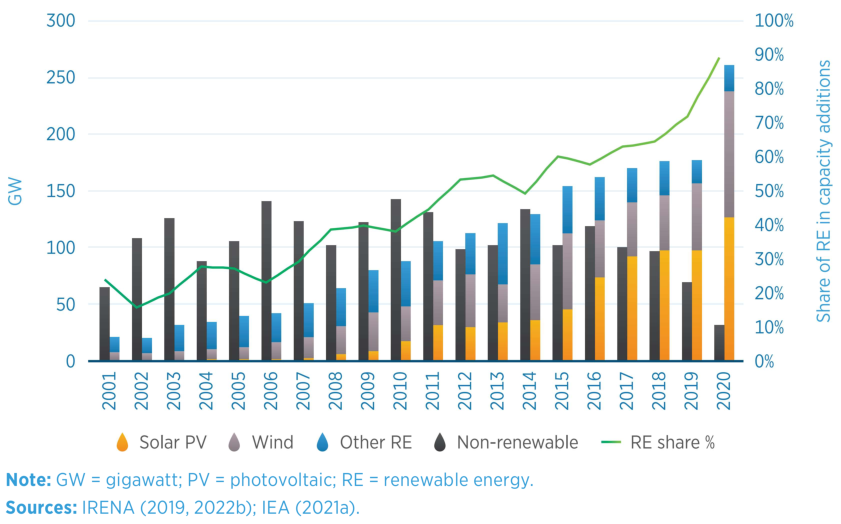
\includegraphics[width=0.8\textwidth]{01_fig_energy_production.pdf}
    \caption{IEA-ETSAP and IRENA© Technology Brief E06 – February 2015}
    \label{fig:production_energy_world}
\end{figure}

Renewable energy refers to energy derived from sources that are naturally restore on a human timescale. Unlike fossil fuels, which are finite and contribute to environmental degradation through greenhouse gas emissions, renewable energy sources are considered cleaner and more sustainable. Common types of renewable energy include solar power, wind power, hydropower, geothermal energy, and biomass. \dtd{lund2007}
Solar power harnesses the energy from the sun through photovoltaic cells, converting sunlight into electricity. Wind power utilizes the kinetic energy of the wind to turn turbines and generate electricity. Hydropower involves capturing the energy from moving water, often through dams or turbines. Geothermal energy taps into the Earth's internal heat for power generation. Biomass, on the other hand, involves converting organic materials such as plants and waste into energy.

The research of this thesis is focused on hydropower energy production. Hydropower stands as a well-established technology currently deployed in approximately 160 countries for the production of cost-effective, low-carbon, and renewable electricity. \dtd{irena}

Hydropower plants exhibit two fundamental configurations: those based on dams with reservoirs and run-of-the-river plants that lack reservoirs. Dams can further be classified into small dams with day-and-night regulation, large dams with seasonal storage, and pumped storage reversible plants capable of both generating and pumping for energy storage, adjusting to the fluctuations in electricity demand. Small-scale hydropower is frequently utilized for rural applications. \dtd{balmer}

With a cumulative capacity reaching around \SI{1060}{GW} (constituting \SI{19.4}{\%} of the world's electric capacity in 2011 \dtd{irena}), hydropower contributes to an annual electricity generation of about \SI{3500}{TWh}, accounting for \SI{15.8}{\%} of the global electricity generation in 2011. In over 35 countries, hydropower plants play a significant role by supplying at least \SI{50}{\%} of the total electricity demand. Italy is one of these countries with an installed capacity around \SI{19}{GW} hydropower plants generates about \SI{199}{TWh}, accounting for \SI{70}{\%} of the total electricity generation in 2022. \dtd{terna}

The optimization of hydropower energy production is one of the step forward the transition to renewable energy with the desire to reduce dependence on fossil fuels, and the recognition of the economic benefits associated with clean energy technologies. \dtd{barros, chun-thian} Governments and organizations worldwide are increasingly focusing on implementing policies and initiatives to promote the adoption of renewable energy and mitigate the impact of climate change.

Indeed, anticipating climate-change-induced changes in rainfall, water flows and extreme weather events is crucial for hydropower development planning as well as adequate power system planning. It is particularly important for governments, operators and decision makers to be aware of the issues that climate change can create on annual run-offs, their time distribution and sedimentation. The IHA produced a Climate Resilience Guide \dtd{Climate Resilience Guide} for the hydropower sector, which offers a methodology for identifying, assessing and managing climate risks to enhance the resilience of hydropower projects.

%% water-nexus means optimize the production maintaining the condition to use the water in other fields (agricultur irrigation) and protect the territories (flood control), and to satisfy the human uses and the quality of the water.

% digitalization
%% one of the main points to do it

%********************************** % Section 1.2 **************************************
\section{The Italian electricity market\label{section1.2}}

The electric market in Italy, established by the Legislative Decree of March 16, 1999, No. 79 (Legislative Decree No. 79/99), is a product of the transposition process of the European directive aiming to create an internal energy market (Directive 96/92/EC). This market is designed to address two specific needs: to promote competition in electricity production and trading and to ensure the economic management of dispatching services with criteria of neutrality, transparency, and objectivity.

The Italian electric market is divided into two main segments: the Spot Electricity Market (MPE) and the Forward Electricity Market (MTE). This research project is featured for the Spot Electricity Market, that further breaks down into the Day-Ahead Market (MGP), the Intraday Market (MI), the Daily Products Market (MPEG), and the Dispatching Service Market (MSD). The goal of the research in this thesis is based on the Day-Ahead Market (MGP).

The Day-Ahead Market (MGP) plays a crucial role in hosting the majority of electricity trading transactions. This market facilitates the exchange of hourly blocks of energy for the next day. The trading session opens at 8:00 am on the ninth day preceding the delivery day and closes at 12:00 pm on the day before the delivery day. The market results are communicated by 12:58 pm on the day before the delivery day.

Operators participate in the MGP by submitting bids that indicate the quantity and the maximum/minimum price at which they are willing to buy or sell electricity. The MGP operates as an auction market rather than a continuous trading market. Accepted bids are determined based on economic merit and within the limits of transit between zones.

The accepted purchase bids related to consumption units belonging to Italian geographical zones are valued at the National Single Price (PUN). The PUN is calculated as the average of the prices of geographical zones weighted by the quantities purchased in those zones. On the other hand, sale bids and purchase bids related to both pumping units and consumption units belonging to foreign virtual zones are valued at the marginal equilibrium price of the respective zones.

The GME (Electricity Market Operator) acts as the central counterparty, facilitating the trading activities in the market. The GME ensures the efficient functioning of the market by managing the acceptance of bids, determining equilibrium prices, and maintaining transparency and fairness in the trading process.

In summary, the Italian electric market, born out of legislative measures in 1999, operates with the aim of fostering competition and ensuring the economic management of dispatching services. The Spot Electricity Market, particularly the Day-Ahead Market, serves as a pivotal platform for electricity trading, with a focus on transparency, objectivity, and economic efficiency. The GME plays a central role in maintaining the integrity of the market, acting as a key intermediary in the trading activities between market participants.

%********************************** % Section 1.3 *************************************
\section{The challenges of this research\label{section1.3}}
% optimization for a sustainable energy production: prediction with confidence of the streamflow for the day-ahead market, with optimized use of the resources 
% digitalization of the meteo-hydro pipeline chain

%********************************** % Section 1.4 *************************************
\section{Region of Interest: the South Tyrol\label{section1.4}}

\subsection{Description of the area}
% description of the posizion, area and climatology
This research primarily concentrated on South Tyrol, a northern Italian Province. South Tyrol is an Alpine area distinguished by high elevation mountains separated by well defined valleys. The predominant geography of this region is influenced by three principal rivers: Adige, Isarco, and Rienza.

% main streams and lakes
The Adige River is the second-longest river in Italy and its catchment is the biggest in South Tyrol. Originating near the Reschen Pass, nestled in the Alps between Italy and Austria, this river courses through the western sector of the province until it reaches Bolzano. It collects here all water from the remaining South Tyrol region. Specifically, the Rienza River, originating at Braies Lake, traverses the Pusteria Valley and converges with the Isarco River near Bressanone. Subsequently, the Isarco River, with its source in the Brenner Pass, flows from north to south and merges with the Adige River in the town of Bolzano. From Bolzano to the hydrological closure of the Bolzano region all the remain water is collected in the Adige river.

In South Tyrol, there are approximately 350 lakes. All these bodies of water, whether in the mountains or on the plains, constitute extraordinary ecosystems that shape the landscape, host a wide variety of habitats for numerous animals and plants, and are therefore crucial for biodiversity conservation. Additionally, their presence adds value to the region as they serve as important recreational areas. The Province of Bolzano has always been committed to protecting this natural heritage and preserving the good quality of water, both chemically and ecologically.

The administrative area of South Tyrol is \SI{7400}{km^2} with elevation spanning from \SI{70}{\elevationunit} in Salorno to \SI{3950}{\elevationunit} of the Ortles peak. The case study climatology is well describes as Alpine, with precipitation and temperature as the main hydrological drivers. Average annual precipitation over the entire South Tyrol region is about \SI{1000}{mm}. In winter, the precipitation is partially retained as snowpack at the highest elevation where the temperature reaches \SI{-35}{\celsius} on the mountain peaks. The snow usually melts in spring and summer when the temperature rises with a maximum registered temperature of \SI{37}{\celsius} in Bolzano. On the other side, precipitation is concentrated mainly in summer and autumn with local and high-intensity storms. In these seasons, the combination of snow melting and higher precipitation event frequency leads to higher streamflow discharge in the rivers.

% population and demands
The population of South Tyrol is about 520000 inhabitants, with more than 200000 inhabitants located in the main cities of the region. The demand of water in this region is mainly divided in human use, agriculture and energy production. Water management in South Tyrol is crucial to ensuring a sustainable balance between water supply and demand. The local authorities through PGUAP and PTA monitor and implement measures to meet the needs of the population while maintaining the health of aquatic ecosystems and preserving water quality.

% energy production


\subsection{Data availability}
% ground stations
% Reanalysis data
% Forecast data
% Data Uncertainties

%********************************** % Section 1.5  *************************************
\section{Hydrological models and data-driven approach\label{section1.5}}  

\subsection{Hydrological models}
% hydrological models as forecaster, pros and cons
\subsection{Data-driven models}
% data-driven models as alternative..pros and cons


%********************************** % Section 1.6 *************************************
\section{Uncertainties propagation\label{section1.6}}  

\subsection{Weather Forecasting ensemble}
% ensemble as result of different initial condition
% ensemble as result of different models

\subsection{Data-driven hydrological ensemble}
% ensemble as result of different input data
% ensemble as result of different models

\subsection{Prediction confidence: uncertainty}
% definition of the confidence
% quantiles as confidence
% confidence as result of ensemble propagation
%!TEX root = ../thesis.tex
%*******************************************************************************
%****************************** Second Chapter *********************************
%*******************************************************************************

\chapter{Reanalysis data and biases}

\ifpdf
    \graphicspath{{Chapter2/Figs/Raster/}{Chapter2/Figs/PDF/}{Chapter2/Figs/}}
\else
    \graphicspath{{Chapter2/Figs/Vector/}{Chapter2/Figs/}}
\fi

%********************************** %Section 2.1 **************************************
\section{Suitability of ERA5-Land reanalysis dataset for hydrological modelling in the Alpine region\label{section2.1}}

% \begin{itemize}
%     \item type of data: ground stations, re-analysis, forecast
%     \item ground stations: problems and perspectives
%     \begin{itemize}
%         \item maintenance
%         \item interpolation methods
%     \end{itemize}
%     \item re-analysis: ERA5, ERA5-Land, VHR-REA\_IT
%     \item 
% \end{itemize}


% \begin{figure}[htbp!] 
% \centering    
% 
\includegraphics[width=1.0\textwidth]{minion}
% \caption[Minion]{This is just a long figure caption for the minion in Despicable Me from Pixar}
% \label{fig:minion}
% \end{figure}


% %********************************** %Section 2.2 **************************************
% \section{Re-analysis data as a reference\label{section2.2}}

% If you have trouble viewing this document contact Krishna at: \href{mailto:kks32@cam.ac.uk}{kks32@cam.ac.uk} or raise an issue at \url{https://github.com/kks32/phd-thesis-template/}




% %********************************** %Section 2.3 **************************************
% \section{Bias correction methods\label{section2.3}}

%!TEX root = ../thesis.tex
%*******************************************************************************
%****************************** Third Chapter **********************************
%*******************************************************************************
\chapter{Modelling uncertainties}

% **************************** Define Graphics Path **************************
\ifpdf
    \graphicspath{{Chapter3/Figs/Raster/}{Chapter3/Figs/PDF/}{Chapter3/Figs/}}
\else
    \graphicspath{{Chapter3/Figs/Vector/}{Chapter3/Figs/}}
\fi

%********************************** %First Section  **************************************
\section{Hydrological models} %Section - 3.1


%********************************** %First Section  **************************************
\section{Econometric models} %Section - 3.2


%********************************** %FSecond Section  **************************************
\section{The multi-model approach} %Section - 3.3

\subsection{Econometric ensemble}
\subsection{Hydrological ensemble}



% \subsection{First subsection in the first section}

% \subsubsection{First subsub section in the third subsection}
% \dots and some more in the first subsub section otherwise it all looks the same
% doesn't it? well we can add some text to it and some more and some more and
% some more and some more and some more and some more and some more \dots

% \subsubsection{Second subsub section in the third subsection}
% \dots and some more in the first subsub section otherwise it all looks the same
% doesn't it? well we can add some text to it \dots

% \section{Second section of the third chapter}
% and here I write more \dots

% \section{The layout of formal tables}
% This section has been modified from ``Publication quality tables in \LaTeX*''
%  by Simon Fear.

% The layout of a table has been established over centuries of experience and 
% should only be altered in extraordinary circumstances. 

% When formatting a table, remember two simple guidelines at all times:

% \begin{enumerate}
%   \item Never, ever use vertical rules (lines).
%   \item Never use double rules.
% \end{enumerate}

% These guidelines may seem extreme but I have
% never found a good argument in favour of breaking them. For
% example, if you feel that the information in the left half of
% a table is so different from that on the right that it needs
% to be separated by a vertical line, then you should use two
% tables instead. Not everyone follows the second guideline:

% There are three further guidelines worth mentioning here as they
% are generally not known outside the circle of professional
% typesetters and subeditors:

% \begin{enumerate}\setcounter{enumi}{2}
%   \item Put the units in the column heading (not in the body of
%           the table).
%   \item Always precede a decimal point by a digit; thus 0.1
%       {\em not} just .1.
%   \item Do not use `ditto' signs or any other such convention to
%       repeat a previous value. In many circumstances a blank
%       will serve just as well. If it won't, then repeat the value.
% \end{enumerate}

% A frequently seen mistake is to use `\textbackslash begin\{center\}' \dots `\textbackslash end\{center\}' inside a figure or table environment. This center environment can cause additional vertical space. If you want to avoid that just use `\textbackslash centering'


% \begin{table}
% \caption{A badly formatted table}
% \centering
% \label{table:bad_table}
% \begin{tabular}{|l|c|c|c|c|}
% \hline 
% & \multicolumn{2}{c}{Species I} & \multicolumn{2}{c|}{Species II} \\ 
% \hline
% Dental measurement  & mean & SD  & mean & SD  \\ \hline 
% \hline
% I1MD & 6.23 & 0.91 & 5.2  & 0.7  \\
% \hline 
% I1LL & 7.48 & 0.56 & 8.7  & 0.71 \\
% \hline 
% I2MD & 3.99 & 0.63 & 4.22 & 0.54 \\
% \hline 
% I2LL & 6.81 & 0.02 & 6.66 & 0.01 \\
% \hline 
% CMD & 13.47 & 0.09 & 10.55 & 0.05 \\
% \hline 
% CBL & 11.88 & 0.05 & 13.11 & 0.04\\ 
% \hline 
% \end{tabular}
% \end{table}

% \begin{table}
% \caption{A nice looking table}
% \centering
% \label{table:nice_table}
% \begin{tabular}{l c c c c}
% \hline 
% \multirow{2}{*}{Dental measurement} & \multicolumn{2}{c}{Species I} & \multicolumn{2}{c}{Species II} \\ 
% \cline{2-5}
%   & mean & SD  & mean & SD  \\ 
% \hline
% I1MD & 6.23 & 0.91 & 5.2  & 0.7  \\

% I1LL & 7.48 & 0.56 & 8.7  & 0.71 \\

% I2MD & 3.99 & 0.63 & 4.22 & 0.54 \\

% I2LL & 6.81 & 0.02 & 6.66 & 0.01 \\

% CMD & 13.47 & 0.09 & 10.55 & 0.05 \\

% CBL & 11.88 & 0.05 & 13.11 & 0.04\\ 
% \hline 
% \end{tabular}
% \end{table}


% \begin{table}
% \caption{Even better looking table using booktabs}
% \centering
% \label{table:good_table}
% \begin{tabular}{l c c c c}
% \toprule
% \multirow{2}{*}{Dental measurement} & \multicolumn{2}{c}{Species I} & \multicolumn{2}{c}{Species II} \\ 
% \cmidrule{2-5}
%   & mean & SD  & mean & SD  \\ 
% \midrule
% I1MD & 6.23 & 0.91 & 5.2  & 0.7  \\

% I1LL & 7.48 & 0.56 & 8.7  & 0.71 \\

% I2MD & 3.99 & 0.63 & 4.22 & 0.54 \\

% I2LL & 6.81 & 0.02 & 6.66 & 0.01 \\

% CMD & 13.47 & 0.09 & 10.55 & 0.05 \\

% CBL & 11.88 & 0.05 & 13.11 & 0.04\\ 
% \bottomrule
% \end{tabular}
% \end{table}

%!TEX root = ../thesis.tex
%*******************************************************************************
%****************************** Third Chapter **********************************
%*******************************************************************************
\chapter{Bias correction methods}

% **************************** Define Graphics Path **************************
\ifpdf
    \graphicspath{{Chapter4/Figs/Raster/}{Chapter4/Figs/PDF/}{Chapter4/Figs/}}
\else
    \graphicspath{{Chapter4/Figs/Vector/}{Chapter4/Figs/}}
\fi

%********************************** %Section 4.1 **************************************
\section{Bias correction of climate model outputs for hydrology: a critical review\label{section4.1}}
% \begin{itemize}
%     \item Description of the pipeline
%     \item Model Averaging
% \end{itemize}

%********************************** %Section 4.2 **************************************
\section{A comprehensive comparison of statistical and machine
learning methods for bias correction of climate model
simulations: application on ERA5-Land across different
temporal resolutions\label{section4.2}}
%!TEX root = ../thesis.tex
%*******************************************************************************
%****************************** Third Chapter **********************************
%*******************************************************************************
\chapter{Discussion and conclusion}

% **************************** Define Graphics Path **************************
\ifpdf
    \graphicspath{{Chapter5/Figs/Raster/}{Chapter5/Figs/PDF/}{Chapter5/Figs/}}
\else
    \graphicspath{{Chapter5/Figs/Vector/}{Chapter5/Figs/}}
\fi

% %********************************** %First Section  **************************************
% \section{Probabilistic pipeline} %Section - 4.1


% %********************************** %First Section  **************************************
% \section{Model averaging} %Section - 4.2


% %********************************** %FSecond Section  **************************************
% \section{Application on Alto Adige} %Section - 4.3
%!TEX root = ../thesis.tex
%*******************************************************************************
%****************************** Third Chapter **********************************
%*******************************************************************************
\chapter{Uncertanty propagation}

% **************************** Define Graphics Path **************************
\ifpdf
    \graphicspath{{Chapter6/Figs/Raster/}{Chapter6/Figs/PDF/}{Chapter5/Figs/}}
\else
    \graphicspath{{Chapter6/Figs/Vector/}{Chapter6/Figs/}}
\fi

% %********************************** %First Section  **************************************
\section{Uncertanty propagation in a data-driven pipeline for the hydro power plants production: the Vernago case study} %Section - 5.1


% %********************************** %Second Section  **************************************
\section{Data-driven water energy management models forced by ensemble weather forecast models outcome} %Section - 5.2
%!TEX root = ../thesis.tex
%*******************************************************************************
%****************************** Seventh Chapter **********************************
%*******************************************************************************
\chapter{Discussion and Conclusions}

% **************************** Define Graphics Path **************************
\ifpdf
    \graphicspath{{Chapter7/Figs/Raster/}{Chapter7/Figs/PDF/}{Chapter7/Figs/}}
\else
    \graphicspath{{Chapter7/Figs/Vector/}{Chapter7/Figs/}}
\fi



% ********************************** Back Matter *******************************
% Backmatter should be commented out, if you are using appendices after References
%\backmatter

% ********************************** Bibliography ******************************
\begin{spacing}{0.9}

% To use the conventional natbib style referencing
% Bibliography style previews: http://nodonn.tipido.net/bibstyle.php
% Reference styles: http://sites.stat.psu.edu/~surajit/present/bib.htm

\bibliographystyle{apalike}
%\bibliographystyle{unsrt} % Use for unsorted references  
%\bibliographystyle{plainnat} % use this to have URLs listed in References
\cleardoublepage
\bibliography{References/references} % Path to your References.bib file


% If you would like to use BibLaTeX for your references, pass `custombib' as
% an option in the document class. The location of 'reference.bib' should be
% specified in the preamble.tex file in the custombib section.
% Comment out the lines related to natbib above and uncomment the following line.

%\printbibliography[heading=bibintoc, title={References}]


\end{spacing}

% ********************************** Appendices ********************************

% \begin{appendices} % Using appendices environment for more functunality

% \include{Appendix1/appendix1}
% \include{Appendix2/appendix2}

% \end{appendices}

% *************************************** Index ********************************
\printthesisindex % If index is present

\end{document}
